
\begin{figure}[t!]
\centering
\fbox{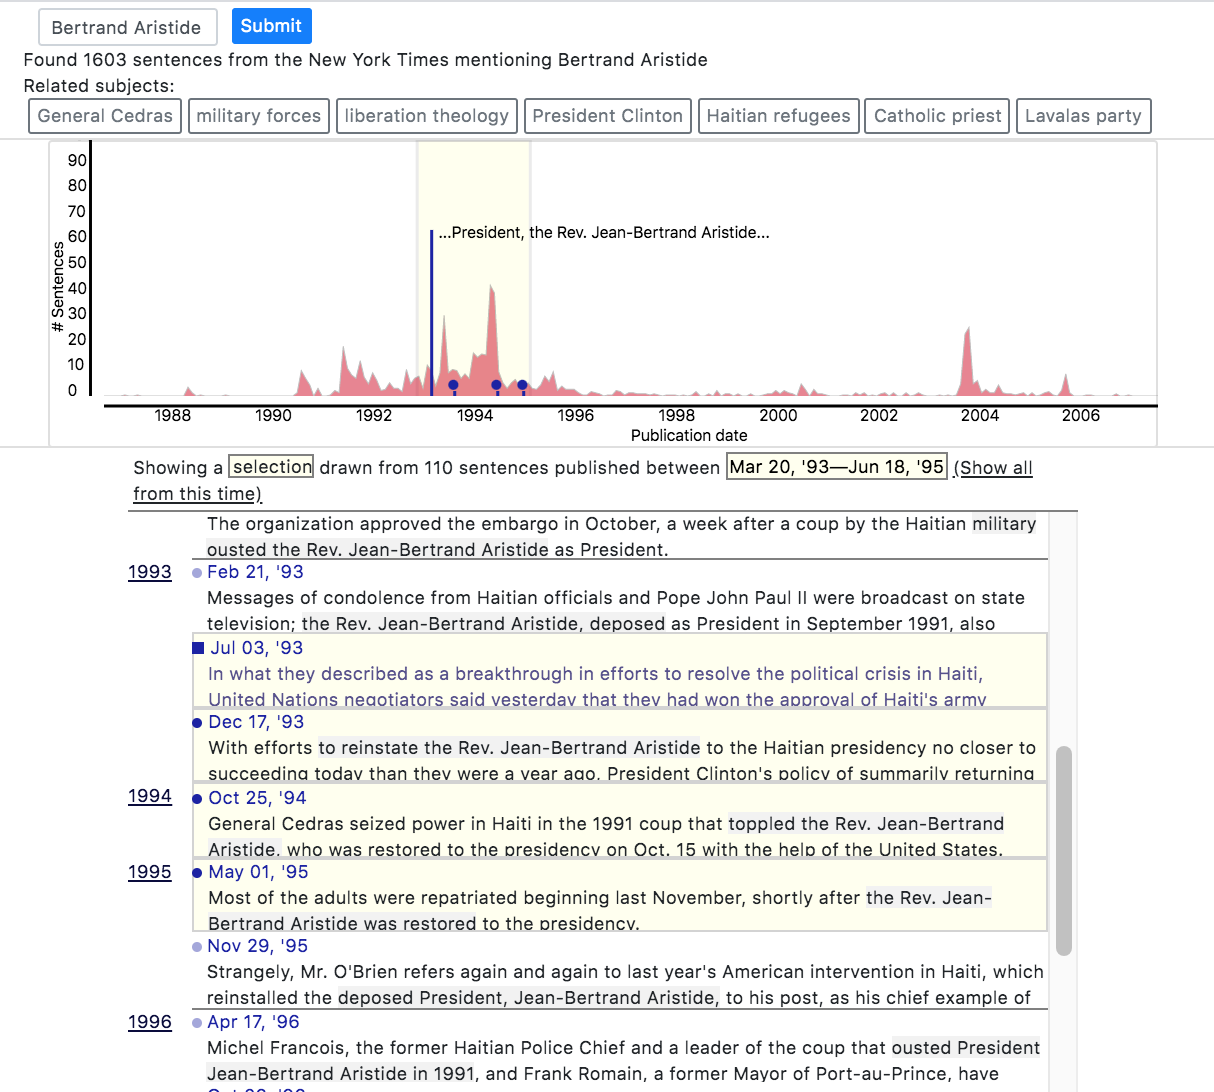
\includegraphics[width=.55\linewidth]{figures/p1.png}}
  \caption[Another early prototype of \ours]{
An early prototype of \ours, which used traditional, optimization-based text summarization methods from natural language processing \cite{McDonald} to try and select the most salient information from a given time period for display. This prototype selects four most ``important'' articles (shaded in light yellow in the feed below), to summarize the hundreds of articles mentioning the query ``Bertrand Aristide'' in \textit{The New York Times} from May 20, '93 to June 18, '95 (shown shaded in light yellow in the time series above).
\ifive~strongly disliked this approach, prompting a shift towards interfaces emphasizing transparency and trustworthiness. 
\textit{``I need to know what is included and why,''} \ifive~ explained. \textit{``I need to know why it is showing this limited view.''} \ifive~continued, \textit{``I am wary of algorithms that choose for me what the important facts are. I am a PhD historian. Leaving stuff out. We are taught to be critical of that.''} Ultimately, \ifive~noted, \textit{``History is written by the victors. What actually matters is what people choose to put in the timeline.''} We theorize that \ifive~could not trust the prototype because it seemed to lack the capacity to select important facts or the integrity to adhere to historical research principles; prior work in HCI (e.g.\ SMILY \cite{smiley}) assumes that in order to earn user trust, a system must both have the capacity to help the user and the integrity to adhere to principles which are important in a given domain.
}\label{f:prototype1}
\end{figure}
